\section{实验进展}
\subsection{MR阻尼器模型设计及理论计算}
\subsubsection{整体结构}
从工作模式来分,MR阻尼器主要有阀式、挤压流动式、剪切式、剪切阀式四种形式;从受力方式来分,可以分为单出杆和双出杆两种类型;从活塞相对于缸体的运动方式来看,可以分为直线型和旋转型。本组采用了剪切阀式、单出杆、直线型MR阻尼器。具体结构分析见图 \ref{mrdamper}。

\begin{figure}[H]
	\centering
	\bicaption{磁流变液阻尼器整体结构}{Overall structure of MR damper}
		{1:端盖; 2:缸壁; 3:线圈挖槽; 4:活塞杆; 5:阻尼通道; 6:磁芯}
		\label{mrdamper}
	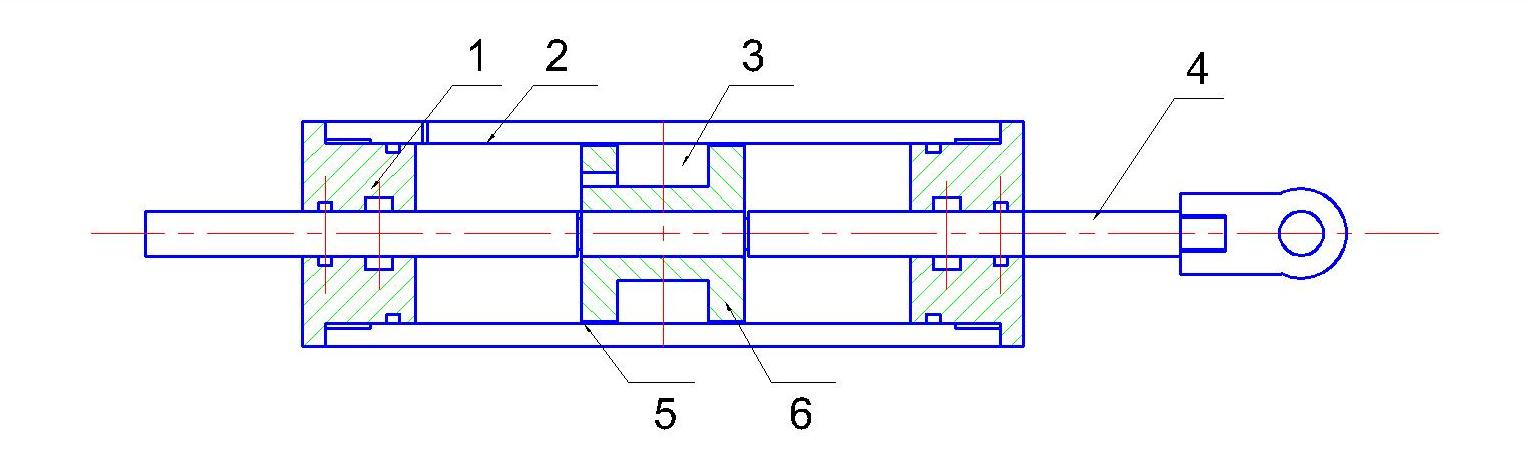
\includegraphics[width=6in]{figure/mrdamper}
\end{figure}

\subsubsection{材料选择}
\paragraph{磁流变液}
\qquad MRF(Magnetorheological fluid)是由大量的顺磁性颗粒悬浮于载体介质(如硅油),并添加一定量的抗沉降和抗凝结的添加剂混合而成。在无外加磁场的情况下,MRF可以简化为经典的牛顿黏性流体。在外加磁场作用下,MRF内部的顺磁性颗粒将发生极化,相互牵引形成链状结构,能够显著提高液体的表现黏度(apparent viscosity),大大增强垂直于磁场方向的液体剪切屈服强度(yield shear strength),且当外加磁场消失后,MRF能够重新转退回牛顿黏性流体。更为重要的是,MRF的剪切屈服强度能够由外加磁场强度的大小精确控制,是制作半主动控制装置的理想材料。

本组采用XXXXXXX,性质见表。

良好的MR阻尼器对MRF的性能有较高的要求:首先,由于MRF分散相粒径粗、比重大,长期静置后MRF中的顺磁性颗粒容易沉降,最终导致MRF丧失流动性功能。因此抗沉降和抗凝结的添加剂的质量和比例需要精确控制;其次,在实际的结构抗震环境中,MR阻尼器要承受的环境激励具有不可预知性,为了提供广泛的控制范围,MRF需要提供低零场黏度和高屈服力。最后,由于MRF在减振过程中受到来回剪切作用,要求MRF具备良好的散热性,且在长期的振动下不分层、不团聚、不发生明显的体积改变。

\paragraph{结构主体材料选取}

\qquad MR阻尼器的主要结构部件包括缸筒、活塞盘、活塞杆、端盖及励磁线圈等。

缸筒、活塞杆不仅是主要的受力构件,也参与阻尼器内部磁回路的组成。XX钢材不仅具备较高的机械强度,能够满足受力需求;同时具备较高的相对磁导率,饱和磁感应强度在1.5T以上,能够满足导磁性能的要求。

活塞盘作为磁回路重要的组成部分,要求材料具备良好的导磁性能,即较高的相对磁导率和饱和磁感应强度。电工纯铁是目前MR阻尼器活塞盘的主流材料。然而由于缺少该实验尺寸下的电工纯铁的标准件,单独加工成本较高。且实际地震波的频率大约在5Hz以内,磁感应强度方向变化慢,因此采用纯钢能够满足其导磁需求。因此采用纯钢作为活塞盘制作材料。

为了减少阻尼器在端盖部分发生漏磁现象,端盖采用不导磁的XX制作。

励磁线圈选用直径较大的漆包线,降低电阻,减少励磁线圈的发热量。

\subsubsection{参数设计}

设计过程中已知参数见表\ref{init}。
\begin{table}[H]
\bicaption{设计参数}{Design parameters}
\centering
\label{init}
\footnotesize
\begin{tabular}{|c|c|c|c|}
\hline 零场黏度$\eta$ & MRF屈服剪切应力$\tau_y$ & MRF饱和磁感应强度$B$ & 磁芯材料饱和磁感应强度$B_1$ \\
\hline $0.2Pa\cdot s$ & $68kPa$ & $0.6B$ & $1.5B$ \\
\hline 最大工作电流$I$ & 活塞最大速度$u$ & 空气磁导率$\mu_0$ & 阻尼通道饱和磁场强度$B_2$ \\
\hline $1.0A$ & $0.03m/s$ & $1.26\times10^{-6}H/m$ & $1.5T$ \\
\hline
\end{tabular}
\end{table}



根据磁路欧姆定律,剪切阀式MR阻尼器的磁路计算公式如式\eqref{NI}:
\begin{equation}
NI=\Phi\left(\frac{L^{'}}{\mu_1S_1}+\frac{2h}{\mu_0S_0}\right)=\Phi\left(R_{m1}+R_{m0}\right) \label{NI}
\end{equation}

式中,$N$为励磁线圈匝数;$I$为最大电流;$\Phi$为回路总磁通;$L^{'}$为磁路平均长度;$h$为阻尼通道宽度;$\mu_0$为空气磁导率;$\mu_1$为磁芯磁导率;$S_1$为磁路平均截面积;$S_0$为阻尼通道处平均截面面积;$R_{m1}$为磁路总磁阻;$R_{m0}$为阻尼通道总磁阻。由于$\mu_0$远小于$\mu_1$,因而$R_{m0}$远大于$R_{m1}$。

考虑磁路最优问题,避免活塞磁芯过早饱和,导致磁路浪费,本文假设间隙处的MRF在最大电流状态下能够达到磁饱和状态,即应满足式\eqref{Phi}。此外,假设磁芯处和阻尼通道处同时达到磁饱和状态,可建立磁路关系如式:
\begin{equation}
\Phi=BS_0\label{Phi}
\end{equation}
式中,$B$为MRF的饱和磁感应强度。

\begin{equation}
\Phi_1=\Phi_2\label{Phi1}
\end{equation}
\begin{equation}
\Phi_1=\pi r^2B_1\label{Phi2}
\end{equation}
\begin{equation}
\Phi_2=2\pi\left(r+h_1\right)L_1B\label{Phi3}
\end{equation}
式中,$\Phi_1$为磁芯处的饱和磁通;$\Phi_2$为阻尼通道处的饱和磁通;$B_1$为磁芯材料的饱和磁感应强度;$r$为磁芯半径;$h_1$为线圈槽挖深;$L_1$为活塞翼缘宽度。

由\eqref{Phi1}简化可得:
\begin{equation}
L_1=\frac{r^2B_1}{2\left(r+h_1\right)B}
\end{equation}

根据式\eqref{Phi},式\eqref{NI}可简化为式\eqref{N}。对于选定的MRF及最大工作电流,励磁线圈匝数$N$仅由阻尼通道宽度$h$确定。
\begin{equation}
N=\frac{2Bh}{\mu_0I}\label{N}
\end{equation}

本文采用剪切阀式直线型MR阻尼器,阻尼力计算公式可简化为:
\begin{equation}
F=F_{\eta}+F_{\tau}=\frac{12\eta LA{_p}{^2}}{\pi Dh^3}v+\frac{3L\tau_yA_p}{h}sgnv\label{F}
\end{equation}

式中:$F_{\eta}$为粘滞力;$F_{\tau}$为库仑阻尼力;$\eta$为MRF的零场黏度;$L$为活塞有效长度,即有效磁极宽度;$A_p$为活塞面积;$h$为活塞与缸体间的阻尼通道间隙;$D$为活塞外径;$\tau_y$为MRF的剪切屈服强度;$v$为活塞相对于缸体的运动速度。粘滞力与磁场强度无关,仅有MRF自身性质及活塞相对于缸体的运动速度有关,不可调控;库仑阻尼力在总阻尼力中比重较大,且可由磁场强度精确控制。

式\eqref{F}中各参数关系复杂,本文没有直接求解,而是编写程序,根据待定参数磁芯半径$r$和阻尼通道宽度$h$自动进行组合、迭代与测试,经过与加工厂商量,考虑模型的实际加工难度和成本,最终确定$r=11mm$、$h=1mm$及各项设计参数,见表\ref{element}。MR阻尼器活塞细部见图\ref{detail}。

\begin{table}[H]
\centering
\bicaption{设计尺寸}{Design size}
\label{element}
\footnotesize
\begin{tabular}{|c|c|c|c|}
\hline 活塞杆半径$r_0$ & 线圈槽挖宽$L_2$ & 活塞节段数$n$ & 磁芯半径$r$ \\
\hline $5mm$ & $20mm$ & $1$ & $11mm$ \\
\hline 阻尼通道宽度$h$ & 线圈槽挖深$h_1$ & 活塞翼缘宽度$L_1$ & 线圈匝数$N$ \\
\hline $1mm$ & $9mm$ & $8mm$ & $487$ \\
\hline

\end{tabular}
\end{table}

\begin{figure}[htb]
	\centering
	\bicaption{活塞细部图}{Detail structure of piston}
	\label{detail}
	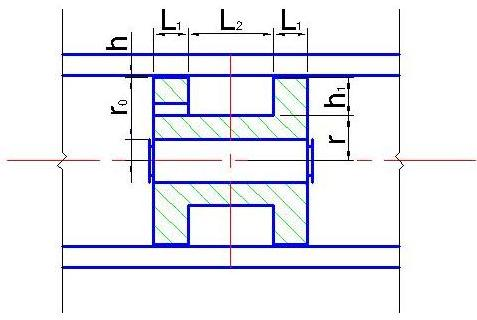
\includegraphics[width=4in]{figure/detail}
\end{figure}

根据表\ref{element}可以进一步计算各项参数如下:
活塞有效长度:
\begin{equation}
L=2nL_1=2\times1\times8mm=16mm
\end{equation}
活塞有效截面积:
\begin{equation}
\begin{split}
A_p&=\pi\left(h_1+r\right)^2-\pi r{_0}{^2}\\&=\pi\times\left(0.009+0.011\right)^2-\pi\times0.005^2=11.78cm^2
\end{split}
\end{equation}
阻尼通道平均周长:
\begin{equation}
\begin{split}
D^{'}&=2\left(r+h_1\right)+h\\&=2\times\left(11+9\right)+1=41mm
\end{split}
\end{equation}

根据式\eqref{F}可得:
\begin{equation}
\begin{split}
F_\eta&=\frac{12\eta LA{_p}{^2}}{\pi Dh^3}v\\&=\frac{12\times0.2\times0.016\times11.78^2\times10^{-4}}{\pi\times0.041\times0.001^3}\times0.03=17.40N
\\
F_{\tau}&=\frac{3L\tau_yA_p}{h}sgnv\\&=\frac{3\times0.016\times68000\times0.1178}{0.001}=3862.71N
\end{split}
\end{equation}

\subsubsection{阻尼器实物}
按照设计的材料、结构和参数,我们联系工厂配置了阻尼液,加工了阻尼器,得到试验用的磁流变阻尼器。

\begin{figure}[H]
	\centering
	\bicaption{磁流变液阻尼器实物}
		{MR damper}
	\label{shiwu}
	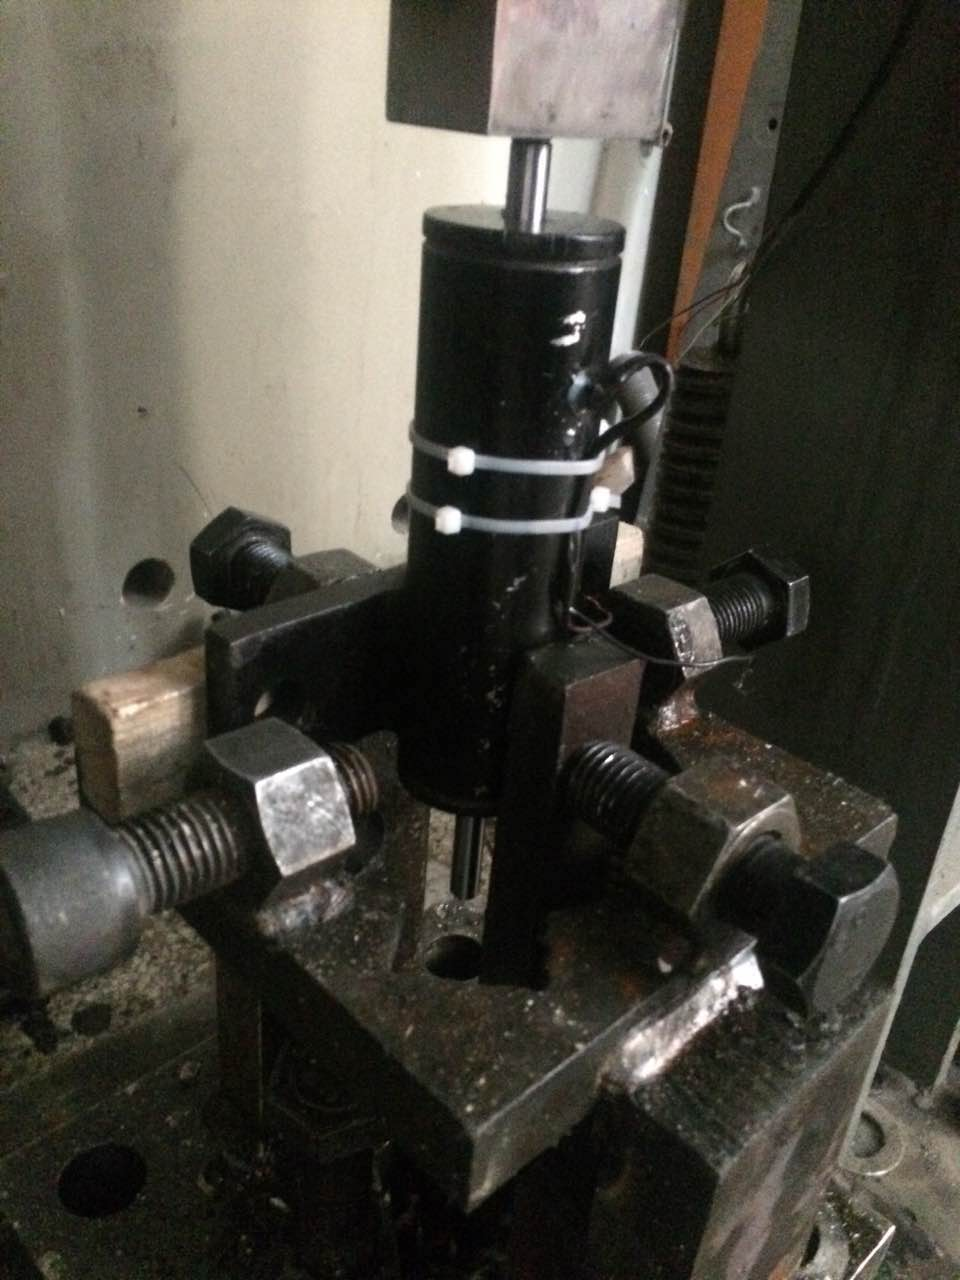
\includegraphics[width=.5\linewidth]{figure/shiwu}
\end{figure}

\subsection{MR阻尼器力学性质测试}

XXXX


\begin{figure}[H]
	\centering
	\bicaption{磁流变液阻尼器滞回曲线测试}
		{Experiment on the hysteresis curve of MR damper}
	\label{shiyan}
	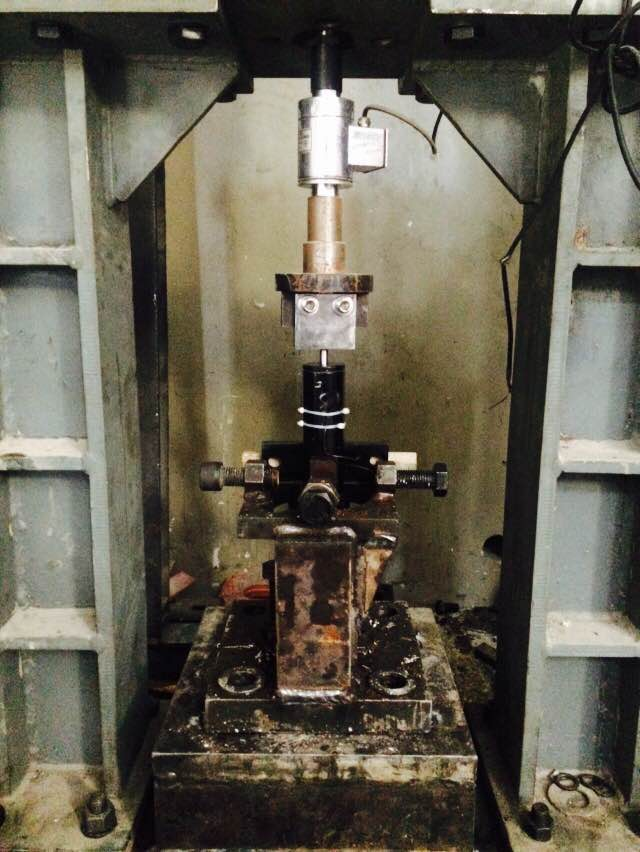
\includegraphics[width=.5\linewidth]{figure/shiyan}
\end{figure}








\subsection{半主动控制系统搭建}

\begin{figure}[H]
	\centering
	\bicaption{中文}
		{English}
	\label{arduino}
	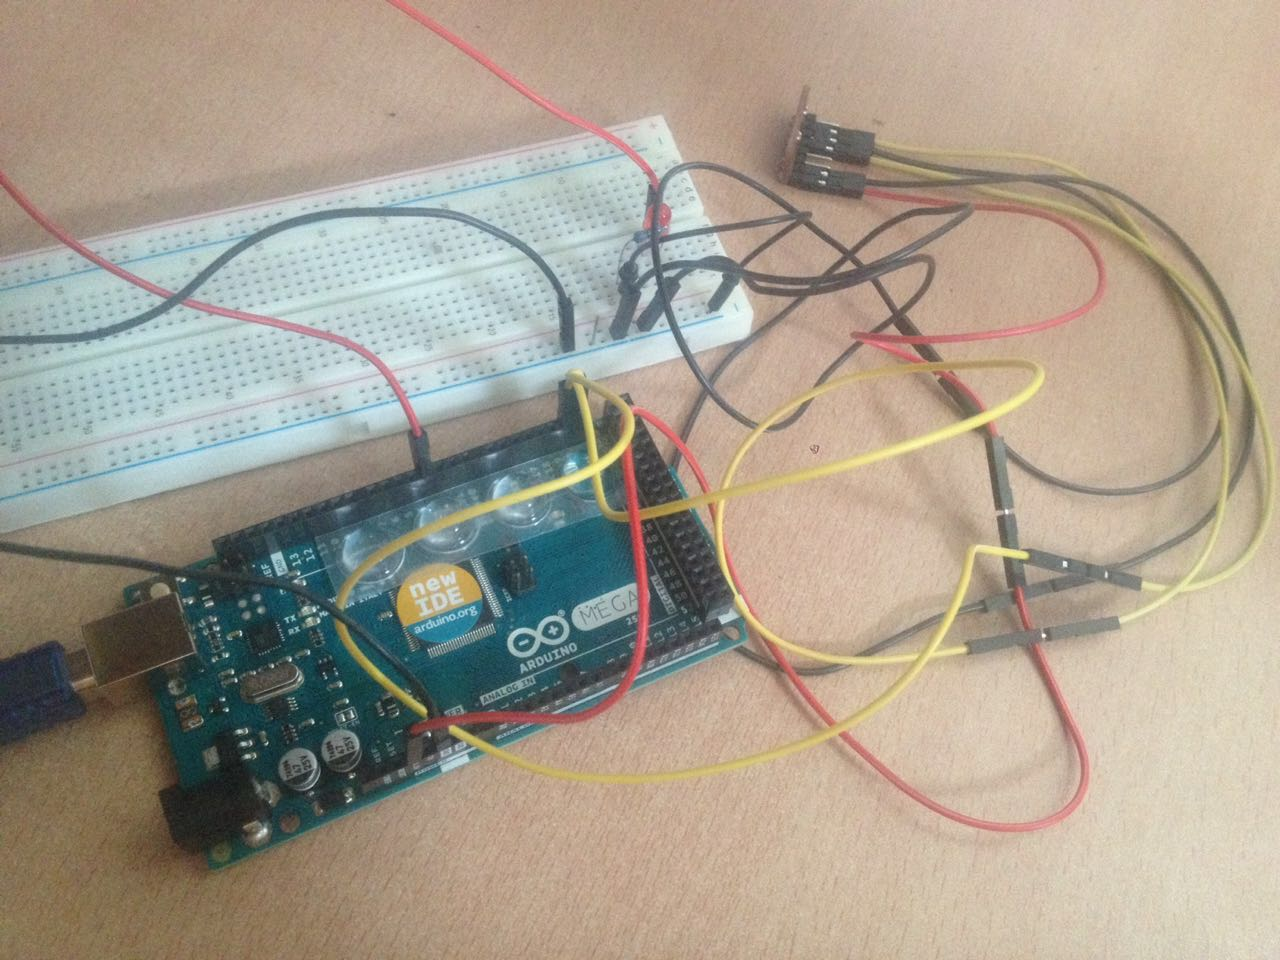
\includegraphics[width=.5\linewidth]{figure/arduino}
\end{figure}




\subsection{直线型发电机设计}
基于法拉第电磁感应定律,闭合回路中的一部分导体,在磁场中运动时,在导体两端会产生感应电动势,并且感应电动势与回路中磁通量的变化率成正比\cite{elliott1993},见式\eqref{magE}。

\begin{equation}
\label{magE}
E=\frac{d\Phi}{dt}
\end{equation}

结合双出型MR阻尼器的机械构造,设计直线型发电机如图\ref{powerstation}所示。该装置由磁漏罩、定子系统与动子系统组成。定子系统包括定子与线圈,线圈绕在定子的凹槽内。动子系统包括永磁体、衔铁与动子连接杆,动子连接杆一头与MR阻尼器双出杆一头相连,永磁体与衔铁相邻布置,为提高发电效率,相邻永磁体极化方向相反,如图XXX所示磁感线近似成矩形。结构在振动时,动子通过动子连接杆与结构连接,与定子产生相对运动,改变线圈内磁通量,从而产生电能。磁漏罩位于装置最外侧,由不导磁材料制成,减少磁漏。

\begin{figure}[H]
\centering
\bicaption{直线型发电机模型}{Linear generator model}
\label{powerstation}
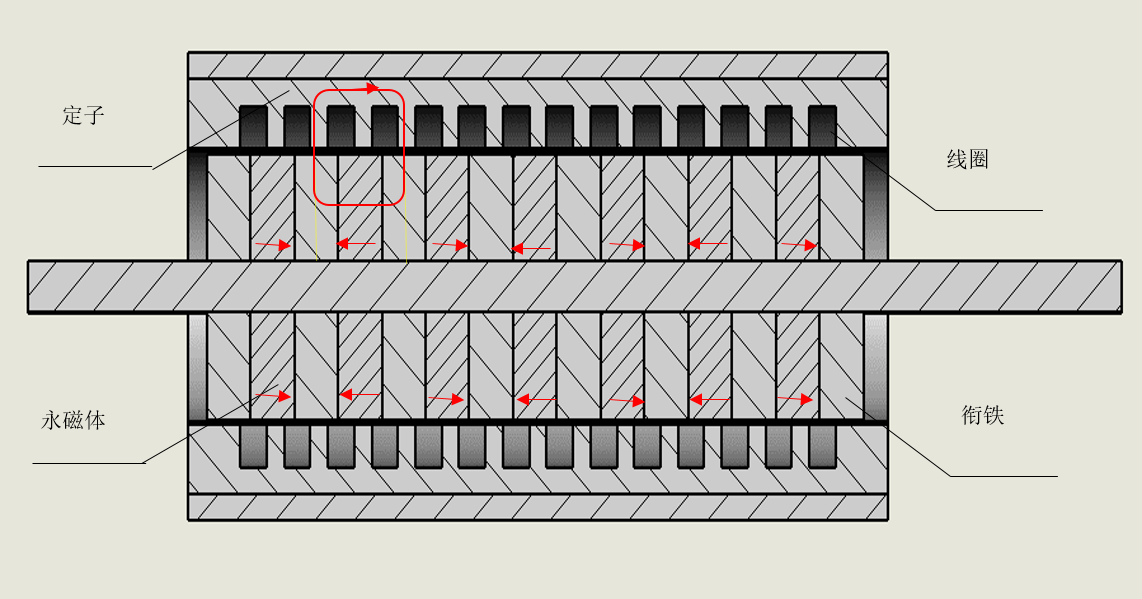
\includegraphics[width=4in]{figure/straight}
\end{figure}

为了能够在低频振动的条件下,收集足够多的电能,在该设计中采取了一系列措施来增大线圈内的磁场强度,防止磁场泄露,提高发电效率:

\begin{enumerate}[leftmargin=*,labelindent=16pt,label=\bfseries \arabic*.]
	\item 采用磁场最强的汝铁硼稀土永磁体材料NdFeB-N50作为永磁体。NdFeB-N50的最大磁能积可达$415kJ/m^3$,利用其产生高强磁场,大大提高发电效率;
	\item 在永磁体排布时,使相邻永磁体极化方向相反,两片永磁体之间用软钢衔铁连接,利用两块永磁体相反的磁动力,迫使磁感线沿装置径向扩散,穿过线圈形成磁回路,提高磁场利用率;
	\item 将线圈分隔成十四个小线圈,每个线圈独立发电,整流后输出电能,充分利用永磁体产生的磁场,提高发电效率;
	\item 设置磁漏罩套于定子外部,磁漏罩由不导磁的铝材料组成,阻止磁感线向外部泄露,迫使磁感线穿越线圈形成闭合回路,用于产生感应电动势。
\end{enumerate}

为进一步验证模型的可行性,在Ansoft Maxwell软件中建立装置模型进行仿真模拟分析。线圈、气隙与塑料筒相对磁导率与真空接近,设置为1;定子及衔铁选用软钢材料,在Maxwell中设置为材料Steel\_1008;磁漏罩与动子连接杆选用不导磁的铝材料,在Maxwell中设置材料为Aluminum;对于永磁体材料,通过自身$B-H$曲线进行定义。

图\ref{simu}所示的是永磁体产生的磁感线在设计装置中的分布图,由模拟结果可见,磁感线的分布与我们设想的基本一致,绝大部分磁感线都能够穿过“气隙—定子T型齿—定子”形成磁感线闭合回路,磁感线形状近似为矩形。当动子与定子产生相对运动时,线圈切割磁力线回路,产生感应电动势。理论仿真所得气隙内磁感应强度平均大小约为$1.157T$,可以达到理论要求。

\begin{figure}[htb]
	\centering
	\bicaption{磁感线分布图}{Distribution map of magnetic induction line}
	\label{simu}
	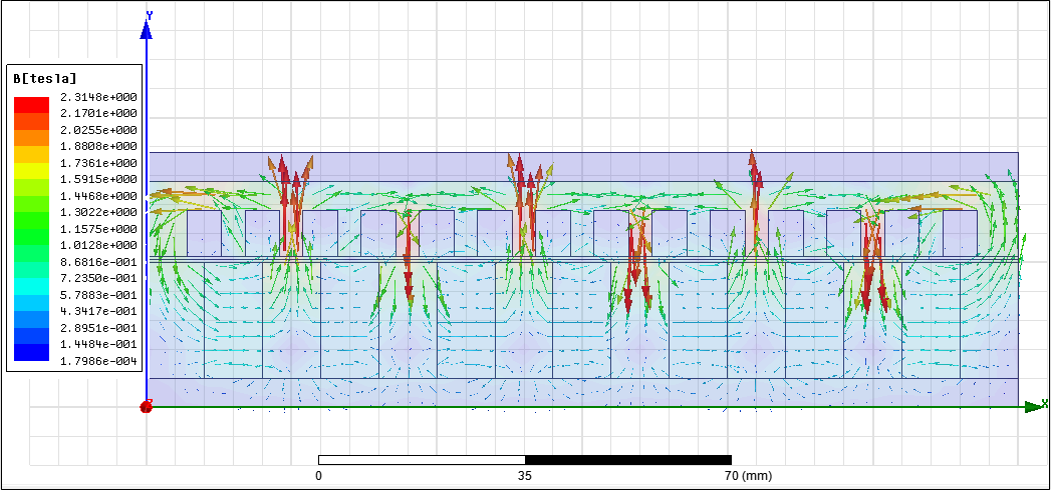
\includegraphics[width=5in]{figure/simu}
\end{figure}

通过理论仿真,我们初步验证了该发电装置的可行性,现阶段该模型已绘制详细图纸交由厂家制作,由于生产过程中存在较多不确定因素,该发电装置的理论发电量计算与试验分析将在后续报告中进行详细阐述。